\documentclass[aspectratio=169, 10pt]{beamer}

\usetheme{metropolis}
\usepackage{booktabs}
\usepackage{amsmath}
\usepackage{graphicx}
\usepackage{caption}
\usepackage[T1]{fontenc}
\usepackage[utf8]{inputenc}

% Colors
\definecolor{mDarkTeal}{HTML}{23373b}
\definecolor{mLightBrown}{HTML}{EB811B}
\definecolor{mGreen}{HTML}{2E8B57}
\definecolor{mRed}{HTML}{C0392B}

\setbeamercolor{progress bar}{fg=mLightBrown}
\setbeamercolor{frametitle}{bg=mDarkTeal}

\graphicspath{{../Ergebnisse/Bilder_Arbeit/}}

\title{Surrogate Modeling of Stokes Flow\\Around Settling Crystals}
\subtitle{FNO vs.\ U-Net: Results Overview}
\author{Paul Baselt}
\date{Betreuergespräch, \today}

\begin{document}

\maketitle

% ─────────────────────────────────────────────────────────────────────────────
\begin{frame}{Motivation \& Ziel}
\begin{columns}
\column{0.55\textwidth}
\textbf{Problem:} Numerische Stokes-Strömungssimulationen für
kristallreiche Magmen sind rechenintensiv.\\[8pt]

\textbf{Ziel:} Zwei datengetriebene Surrogatmodelle vergleichen, die
das Stromfunktionsfeld $\psi$ direkt aus der Kristall\-konfiguration
vorhersagen:
\begin{itemize}
  \item \textbf{FNO} – Fourier Neural Operator (spektral, global)
  \item \textbf{U-Net} – Convolutional Encoder–Decoder (lokal)
\end{itemize}
\vspace{6pt}
\textbf{Eingabe:} 5 Kanäle auf $256\!\times\!256$ Gitter\\
(Maske, SDF, Radius, $x$-Koord., $z$-Koord.)\\[4pt]
\textbf{Ausgabe:} $\hat\psi \in \mathbb{R}^{256\times256}$

\column{0.42\textwidth}
\textbf{Verlustfunktion:}
\[
  \mathcal{L} = \underbrace{\mathrm{MSE}(\hat\psi,\psi)}_{\text{Punktgenauigkeit}}
  + \alpha_\text{grad}\underbrace{\mathcal{L}_\text{grad}}_{\text{Gradienten}}
  + \alpha_\text{bnd}\underbrace{\mathcal{L}_\text{bnd}}_{\text{Randbed.}}
\]
$\alpha_\text{grad}$: lineares Ramp-up 0→0.1 in Epoche 1–5\\
$\alpha_\text{bnd} = 0.01$ (fest)\\[6pt]
Hardware: NVIDIA A100 GPU
\end{columns}
\end{frame}

% ─────────────────────────────────────────────────────────────────────────────
\begin{frame}{Warum Stromfunktion? — Analytische Divergenzfreiheit}
\begin{columns}
\column{0.52\textwidth}
\textbf{Inkompressibilitätsbedingung} (Stokes-Strömung):
\[
  \nabla \cdot \mathbf{u} = \frac{\partial u_x}{\partial x} + \frac{\partial u_z}{\partial z} = 0
\]
\vspace{4pt}
\textbf{Stromfunktion $\psi$} — Definition der Geschwindigkeit:
\[
  u_x = \frac{\partial \psi}{\partial z}, \qquad
  u_z = -\frac{\partial \psi}{\partial x}
\]
\vspace{4pt}
\textbf{Nachweis der Divergenzfreiheit:}
\[
  \nabla \cdot \mathbf{u}
    = \frac{\partial^2 \psi}{\partial x \partial z}
    - \frac{\partial^2 \psi}{\partial z \partial x}
    = 0 \quad \checkmark
\]
Gilt für \emph{jede} glatte Funktion $\psi$
\column{0.44\textwidth}
\textbf{Konsequenzen für das Surrogatmodell:}
\begin{itemize}
  \item Divergenz-RMS aller FNO-Vorhersagen: $\sim10^{-26}$
  \item Physikalische Konsistenz analytisch garantiert —
        kein expliziter Divergenz-Strafterm nötig
  \item Geschwindigkeit aus $\psi$ per Finite-Differenzen:
        Fehler in $\psi$ werden durch Ableitung \emph{verstärkt}\\
        $\Rightarrow$ Gradient-Loss reduziert Hochfrequenzartefakte
\end{itemize}
\end{columns}
\end{frame}

% ─────────────────────────────────────────────────────────────────────────────
\begin{frame}{Experimentübersicht}
\begin{table}
\small
\begin{tabular}{llll}
\toprule
\textbf{Exp.} & \textbf{Training} & \textbf{OOD-Evaluation} & \textbf{Epochen} \\
\midrule
1 – Einzelkristall-Baseline    & $n=1$, $r=0.05$                  & --                       & FNO: 100, U-Net: 180 \\
2 – Mehrkristall-General.      & $n\in\{1,\ldots,10\}$            & $n=11\ldots25$           & FNO: 100, U-Net: 180 \\
3 – Stress-Test                & $n\in\{1,\ldots,25\}$            & $n=30\ldots84$           & FNO: 100, U-Net: 180 \\
4a – Größen-Baseline           & Modell aus Exp.\,1 ($r=0.05$)   & $r=0.005$, $r=0.5$       & kein Training \\
4b – Variable-Radius (FNO)     & $r\in\{0.02, 0.05, 0.08\}$      & $r=0.035, 0.075$ (Interp.)& 100 \\
                               &                                  & $r=0.01, 0.1$ (Extrap.)  &     \\
\bottomrule
\end{tabular}
\end{table}
\vspace{4pt}
Je 1\,000 Training / 100 Validierung / 10 Evaluation Samples pro Stratum (Exp.\,1–3).
Hyperparameter-Suche in Exp.\,1: 4 Lernraten $\times$ 2 Batch-Größen $= 8$ Konfigs pro Modell.
\end{frame}

% ─────────────────────────────────────────────────────────────────────────────
\begin{frame}{Experiment 1: Einzelkristall-Baseline}
\textbf{Beste Konfigurationen} (10 Eval-Samples):
\begin{table}
\small
\begin{tabular}{llcc}
\toprule
\textbf{Modell} & \textbf{Konfig} & $\bar\varepsilon_\psi$ & $\bar\varepsilon_v$ \\
\midrule
\textbf{FNO}   & $5\!\times\!10^{-4}$, bs\,16 & \textbf{1.62\%} & \textbf{3.44\%} \\
FNO            & $5\!\times\!10^{-3}$, bs\,8  & 2.07\% & 4.13\% \\
\midrule
U-Net          & $5\!\times\!10^{-3}$, bs\,8  & 5.5\%  & 8.5\%  \\
U-Net          & $1\!\times\!10^{-4}$, bs\,16            & 13.5\% & 23.1\% \\
\bottomrule
\end{tabular}
\end{table}
\vspace{4pt}
\begin{itemize}
  \item FNO: $\mathbf{3.4\times}$ besser als U-Net auf $\psi$
  \item Gradient-Loss: Verhältnis $\varepsilon_v/\varepsilon_\psi$\\
        von $\sim3\times$ auf $\sim1.5\text{–}2\times$ reduziert
  \item FNO: bs\,16 $>$ bs\,8;\quad U-Net: bs\,8 $\gg$ bs\,16
\end{itemize}

\end{frame}

\begin{frame}{Experiment 1: Einzelkristall-Baseline}
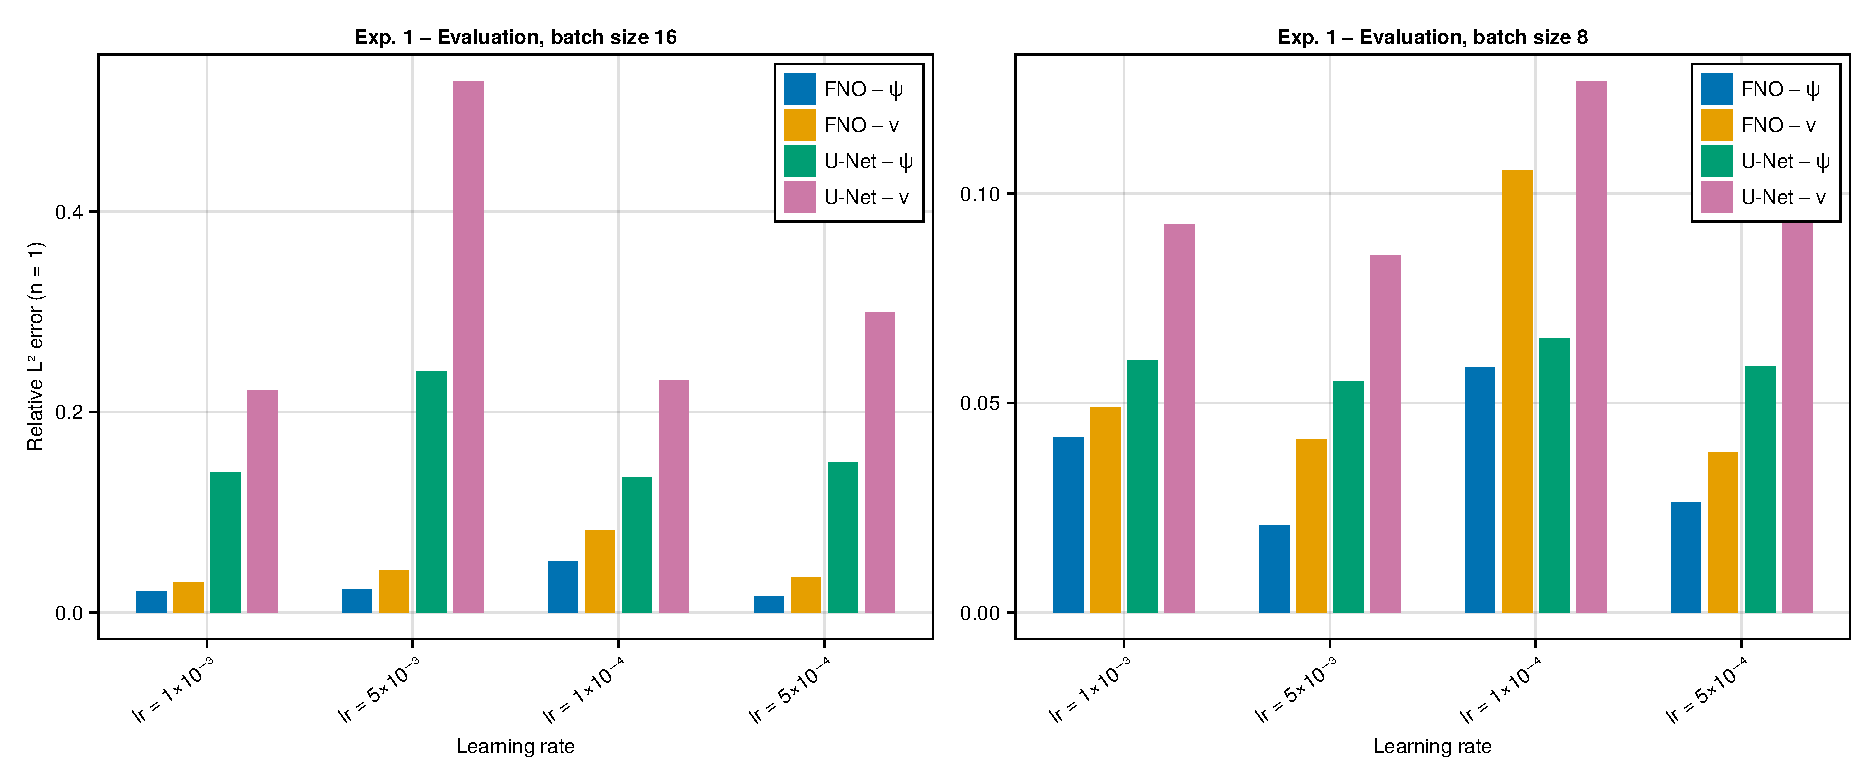
\includegraphics[width=\textwidth]{fig3_exp1_eval_balken.pdf}
\captionof*{figure}{\small Evaluierungsfehler aller lr-Konfigurationen (bs\,16 links, bs\,8 rechts).}
\end{frame}

% ─────────────────────────────────────────────────────────────────────────────
\begin{frame}{Experiment 1: Qualitative Vorhersage (FNO, bs\,16)}
\vspace{-4pt}
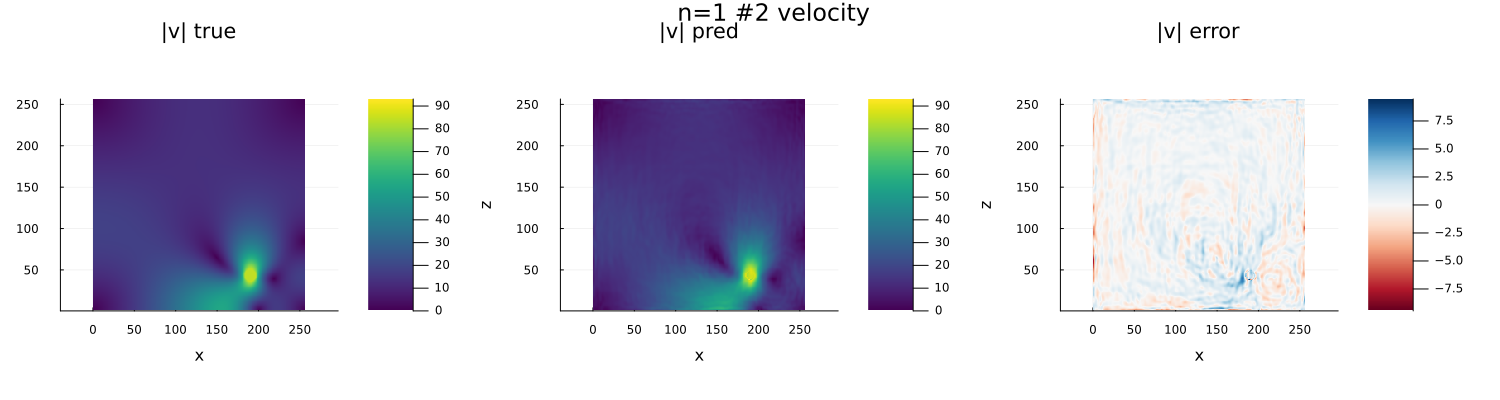
\includegraphics[width=\textwidth]{FNO_Bilder/Exp_1_16_5e-4_psi_vel.png}
\captionof*{figure}{\small FNO Exp-1.4 ($5\!\times\!10^{-4}$, bs\,16): Stromfunktion $\psi$ und Geschwindigkeitsbetrag $|\mathbf{u}|$ — Vorhersage vs.\ numerische Referenz, unnormalisiert.}
\end{frame}

% ─────────────────────────────────────────────────────────────────────────────
\begin{frame}{Experiment 2 \& 3: Mehrkristall-Generalisierung}
\begin{columns}
\column{0.48\textwidth}
\textbf{Exp.\,2} (Training $n\leq10$, FNO: 100\,Ep., U-Net: 180\,Ep.):
\begin{table}
\small
\begin{tabular}{lcc}
\toprule
\textbf{Modell} & $\varepsilon_\psi^\text{in-dist}$ & $\varepsilon_\psi^{n=25}$ \\
\midrule
FNO   & $\sim5.5\%$ & $13.8\%$ \\
U-Net & $\sim22\%$  & $26.8\%$ \\
\bottomrule
\end{tabular}
\end{table}
\vspace{8pt}
\textbf{Exp.\,3} (Training $n\leq25$, FNO: 100\,Ep., U-Net: 180\,Ep.):
\begin{table}
\small
\begin{tabular}{lcc}
\toprule
\textbf{Modell} & $\varepsilon_\psi^\text{in-dist}$ & $\varepsilon_\psi^{n=50}$ \\
\midrule
FNO   & $\sim6.8\%$ & $12.4\%$ \\
U-Net & $\sim23\%$  & $21.5\%$ \\
\bottomrule
\end{tabular}
\end{table}

\column{0.48\textwidth}
\begin{itemize}
  \item FNO: $\mathbf{3\text{–}4\times}$ besser in-dist.
  \item U-Net saturiert früh (Ep.\,43/49, $\sim28\%$)\\
        $\Rightarrow$ kein Vorteil durch längeres Training
  \item Größeres Trainingsset ($n\leq25$) verlängert FNO-Generalisierungsbereich deutlich:\\
        bis $n=30$ kaum Degradation
  \item OOD-Vorteil FNO: $2\times$ bei $n=25$,\\
        $1.7\times$ bei $n=50$
\end{itemize}
\end{columns}
\end{frame}

\begin{frame}{Exp.\,2 \& 3: FNO-Generalisierung über Kristallzahl}
\vspace{-2pt}
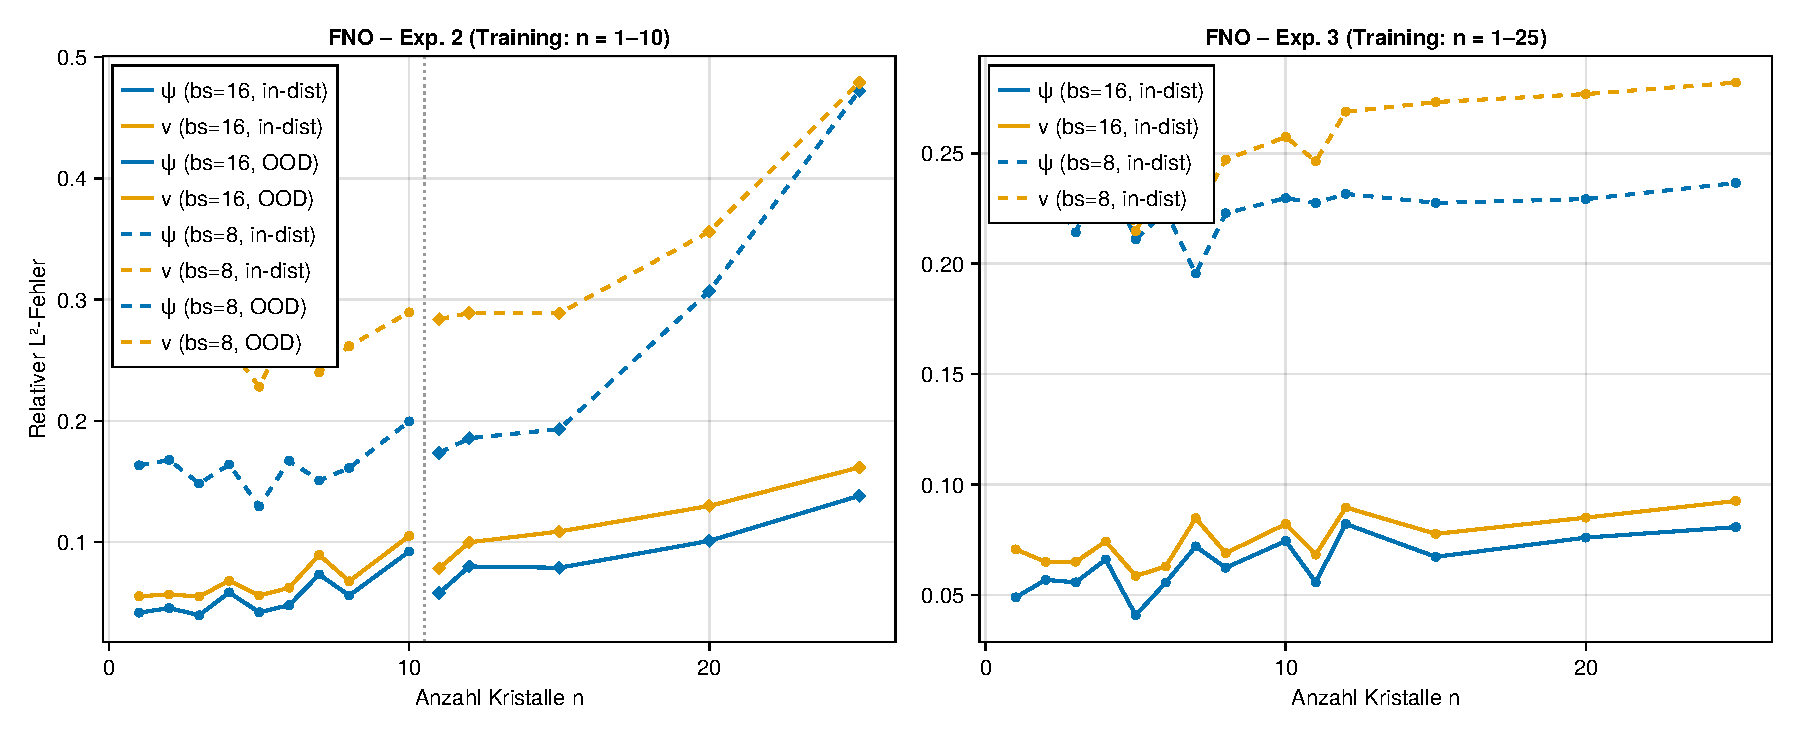
\includegraphics[width=\textwidth]{fig4_fno_exp23_generalisierung.pdf}
\captionof*{figure}{\small FNO: relativer $L_2$-Fehler auf $\psi$ vs.\ Kristallzahl für Exp.\,2 (links, Training $n\leq10$) und Exp.\,3 (rechts, Training $n\leq25$). Gestrichelt = OOD. Vertikale Linie: Trainingsgrenze.}
\end{frame}

\begin{frame}{Exp.\,2 \& 3: U-Net-Generalisierung über Kristallzahl}
\vspace{-2pt}
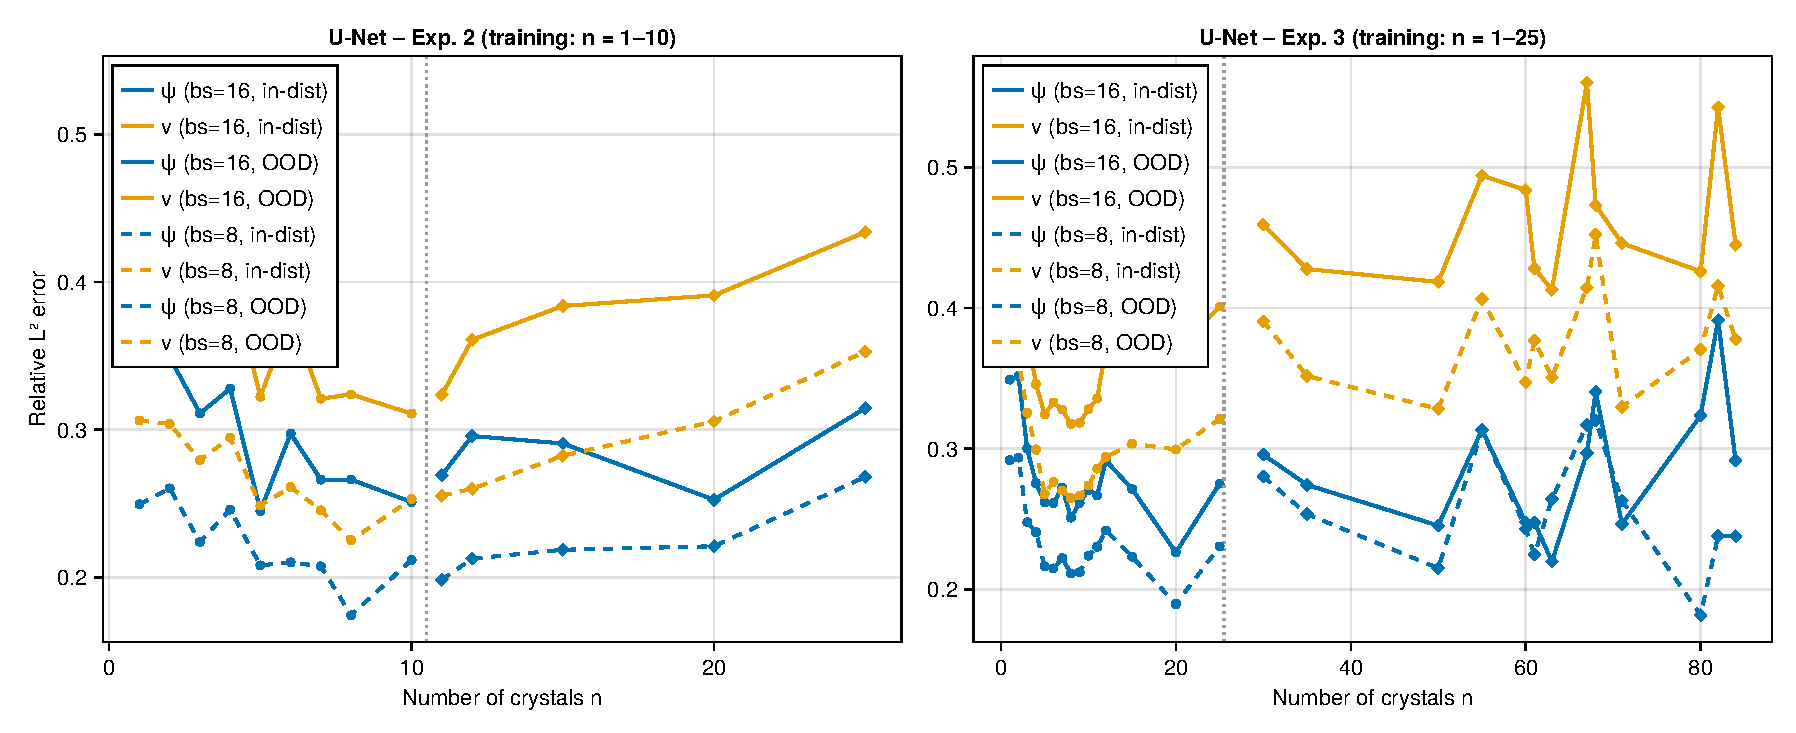
\includegraphics[width=\textwidth]{fig10_unet_exp23_generalisierung.pdf}
\captionof*{figure}{\small U-Net: relativer $L_2$-Fehler auf $\psi$ vs.\ Kristallzahl für Exp.\,2 (links) und Exp.\,3 (rechts). Fehler bleiben durchgehend hoch; Differenz zwischen in-dist.\ und OOD ist gering.}
\end{frame}

% ─────────────────────────────────────────────────────────────────────────────
\begin{frame}{Experiment 4a: Kristallgröße — Fixed-Radius Baseline}
\textbf{Setup:} Bestes Modell aus Exp.\,1 (trainiert auf $r=0.05$) wird ohne Neutraining auf OOD-Größen evaluiert.\\[8pt]
\begin{table}
\small
\begin{tabular}{llcc}
\toprule
\textbf{Modell} & \textbf{Radius} & $\bar\varepsilon_\psi$ & $\bar\varepsilon_v$ \\
\midrule
FNO   & klein ($r=0.005$) & $12.1\%$ & $20.4\%$ \\
\alert{FNO}   & \alert{groß ($r=0.5$)} & \alert{$71.3\%$} & \alert{$67.7\%$} \\
\midrule
U-Net & klein ($r=0.005$) & $10.8\%$ & $20.1\%$ \\
U-Net & groß ($r=0.5$) & $44.9\%$ & $50.7\%$ \\
\bottomrule
\end{tabular}
\end{table}
\vspace{8pt}
\begin{itemize}
  \item \textbf{Kleine Kristalle:} globales Strömungsfeld dominiert — beide Architekturen robust
  \item \textbf{Große Kristalle:} FNO versagt — hohe Ortsfrequenzen nahe der Grenzfläche übersteigen $k_\text{max}=16$
  \item U-Net hier besser — lokale Faltungen besser geeignet für scharfe räumliche Gradienten
\end{itemize}
\end{frame}

\begin{frame}{Exp.\,4a: Größen-Generalisierung (Fixed-Radius)}
\vspace{-2pt}
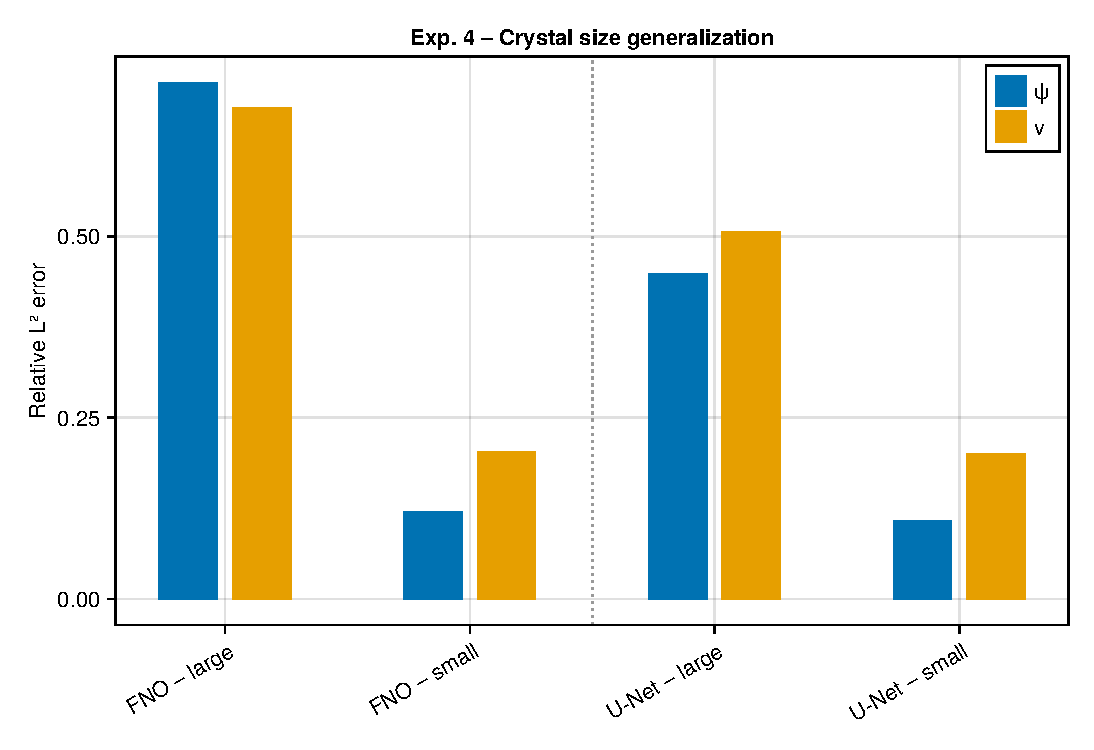
\includegraphics[width=0.7\textwidth]{fig11_exp4_kristallgroesse.pdf}
\captionof*{figure}{\small Relativer $L_2$-Fehler auf $\psi$ und $|\mathbf{u}|$ für FNO und U-Net auf kleinen ($r=0.005$) und großen ($r=0.5$) Kristallen. Training: $r=0.05$.}
\end{frame}

% ─────────────────────────────────────────────────────────────────────────────
\begin{frame}{Experiment 4b: Kristallgröße — Variable-Radius FNO}
\begin{columns}
\column{0.50\textwidth}
\textbf{Setup:} Neues FNO trainiert auf $r\in\{0.02, 0.05, 0.08\}$\\
(je 1\,000 Samples, 100\,Epochen, bs\,16, lr\,$=5\times10^{-4}$)\\[6pt]

\textbf{Evaluation auf 70 Samples:}
\begin{itemize}
  \item In-Distribution: $r=0.02$, $r=0.08$
  \item Interpolation: $r=0.035$, $r=0.075$
  \item Extrapolation: $r=0.01$, $r=0.1$
\end{itemize}
\vspace{6pt}
\begin{table}
\small
\begin{tabular}{lcc}
\toprule
\textbf{Modell} & $\bar\varepsilon_\psi$ & $\bar\varepsilon_v$ \\
\midrule
FNO var.-Radius (gesamt) & $10.35\%$ & $11.63\%$ \\
\midrule
Vergleich: FNO fix, groß OOD & $71.3\%$ & $67.7\%$ \\
\bottomrule
\end{tabular}
\end{table}

\column{0.46\textwidth}
\textbf{Schlüsselergebnis:}
\begin{itemize}
  \item Radius-Eingangskanal ermöglicht Konditionierung auf Geometrie
  \item Hohe Streuung ($\pm10.8\%$) — Extrapolationsradien ($r=0.01$, $r=0.1$) treiben den Fehler
  \item In-Distribution \& Interpolation: deutlich besser als Extrapolation
\end{itemize}
\end{columns}
\end{frame}

% ─────────────────────────────────────────────────────────────────────────────
\begin{frame}{Zusammenfassung \& Fazit}
\begin{columns}
\column{0.50\textwidth}
\textbf{FNO übertrifft U-Net in fast allen Szenarien:}
\begin{table}
\small
\begin{tabular}{lcc}
\toprule
& FNO & U-Net \\
\midrule
Exp\,1 (in-dist.)   & $1.62\%$ & $5.5\%$ \\
Exp\,2 (in-dist.)   & $\sim5.5\%$ & $\sim22\%$ \\
Exp\,2 OOD $n=25$   & $13.8\%$ & $26.8\%$ \\
Exp\,3 (in-dist.)   & $\sim6.8\%$ & $\sim23\%$ \\
Exp\,3 OOD $n=50$   & $12.4\%$ & $21.5\%$ \\
\midrule
Exp\,4a groß OOD    & \alert{$71.3\%$} & $44.9\%$ \\
\bottomrule
\end{tabular}
\end{table}
\vspace{4pt}
\textbf{Ausnahme:} Große Kristalle — U-Net robuster\\durch lokale Faltungsarchitektur.

\column{0.46\textwidth}
\textbf{Schlüsselerkenntnisse:}
\begin{itemize}
  \item Stromfunktions-Ausgabe $\Rightarrow$ Divergenzfreiheit analytisch garantiert
  \item Gradient-Loss reduziert $\varepsilon_v/\varepsilon_\psi$-Verhältnis von $3\times$ auf $1.5\text{–}2\times$
  \item FNO konvergiert stabil; U-Net saturiert früh ($\sim$Ep.\,43–49) bei Mehrkristall-Aufgaben
  \item Breiteres Trainingsset verlängert OOD-Generalisierungsbereich deutlich
  \item Variable-Radius-Training löst Größen-OOD-Problem
\end{itemize}
\end{columns}
\end{frame}

\end{document}
